% --------------------------------------------------------------
% This is all preamble stuff that you don't have to worry about.
% Head down to where it says "Start here"
% --------------------------------------------------------------

\documentclass[12pt]{article}

\usepackage[margin=1in]{geometry}
\usepackage{amsmath,amsthm,amssymb}
\usepackage{graphicx} %This allows to include eps figures
\usepackage{subcaption}
\usepackage[section]{placeins}
\usepackage{layout}
\usepackage{etoolbox}
\usepackage{mathabx}
\usepackage{animate}
\usepackage{array}
% This is to include code
\usepackage{listings}
\usepackage{xcolor}
\definecolor{dkgreen}{rgb}{0,0.6,0}
\definecolor{gray}{rgb}{0.5,0.5,0.5}
\definecolor{mauve}{rgb}{0.58,0,0.82}
\lstdefinestyle{Python}{
    language        = Python,
    basicstyle      = \ttfamily,
    keywordstyle    = \color{blue},
    keywordstyle    = [2] \color{teal}, % just to check that it works
    stringstyle     = \color{green},
    commentstyle    = \color{red}\ttfamily
}

\newenvironment{conditions}
  {\par\vspace{\abovedisplayskip}\noindent\begin{tabular}{>{$}l<{$} @{${}={}$} l}}
  {\end{tabular}\par\vspace{\belowdisplayskip}}

\newcommand{\N}{\mathbb{N}}
\newcommand{\Z}{\mathbb{Z}}

\newenvironment{theorem}[2][Theorem]{\begin{trivlist}
\item[\hskip \labelsep {\bfseries #1}\hskip \labelsep {\bfseries #2.}]}{\end{trivlist}}
\newenvironment{lemma}[2][Lemma]{\begin{trivlist}
\item[\hskip \labelsep {\bfseries #1}\hskip \labelsep {\bfseries #2.}]}{\end{trivlist}}
\newenvironment{exercise}[2][Exercise]{\begin{trivlist}
\item[\hskip \labelsep {\bfseries #1}\hskip \labelsep {\bfseries #2.}]}{\end{trivlist}}
\newenvironment{reflection}[2][Reflection]{\begin{trivlist}
\item[\hskip \labelsep {\bfseries #1}\hskip \labelsep {\bfseries #2.}]}{\end{trivlist}}
\newenvironment{proposition}[2][Proposition]{\begin{trivlist}
\item[\hskip \labelsep {\bfseries #1}\hskip \labelsep {\bfseries #2.}]}{\end{trivlist}}
\newenvironment{corollary}[2][Corollary]{\begin{trivlist}
\item[\hskip \labelsep {\bfseries #1}\hskip \labelsep {\bfseries #2.}]}{\end{trivlist}}



\begin{document}

% --------------------------------------------------------------
%                         Start here
% --------------------------------------------------------------

%\renewcommand{\qedsymbol}{\filledbox}

\title{Assignment 5 - Appendix}%replace X with the appropriate number
\author{Nalet Meinen and Pascal Wyss\\ %replace with your name
Finite Element Analysis I
}
\maketitle

\section{Methods}

In the previous version of this assignment false dimensions were used, resulting in different forces on the plate on the overshooting as commented in the last report. With the correct values and dimension, a better result could be found.

\section{Results}


\begin{figure}[!htb]
  \centering
  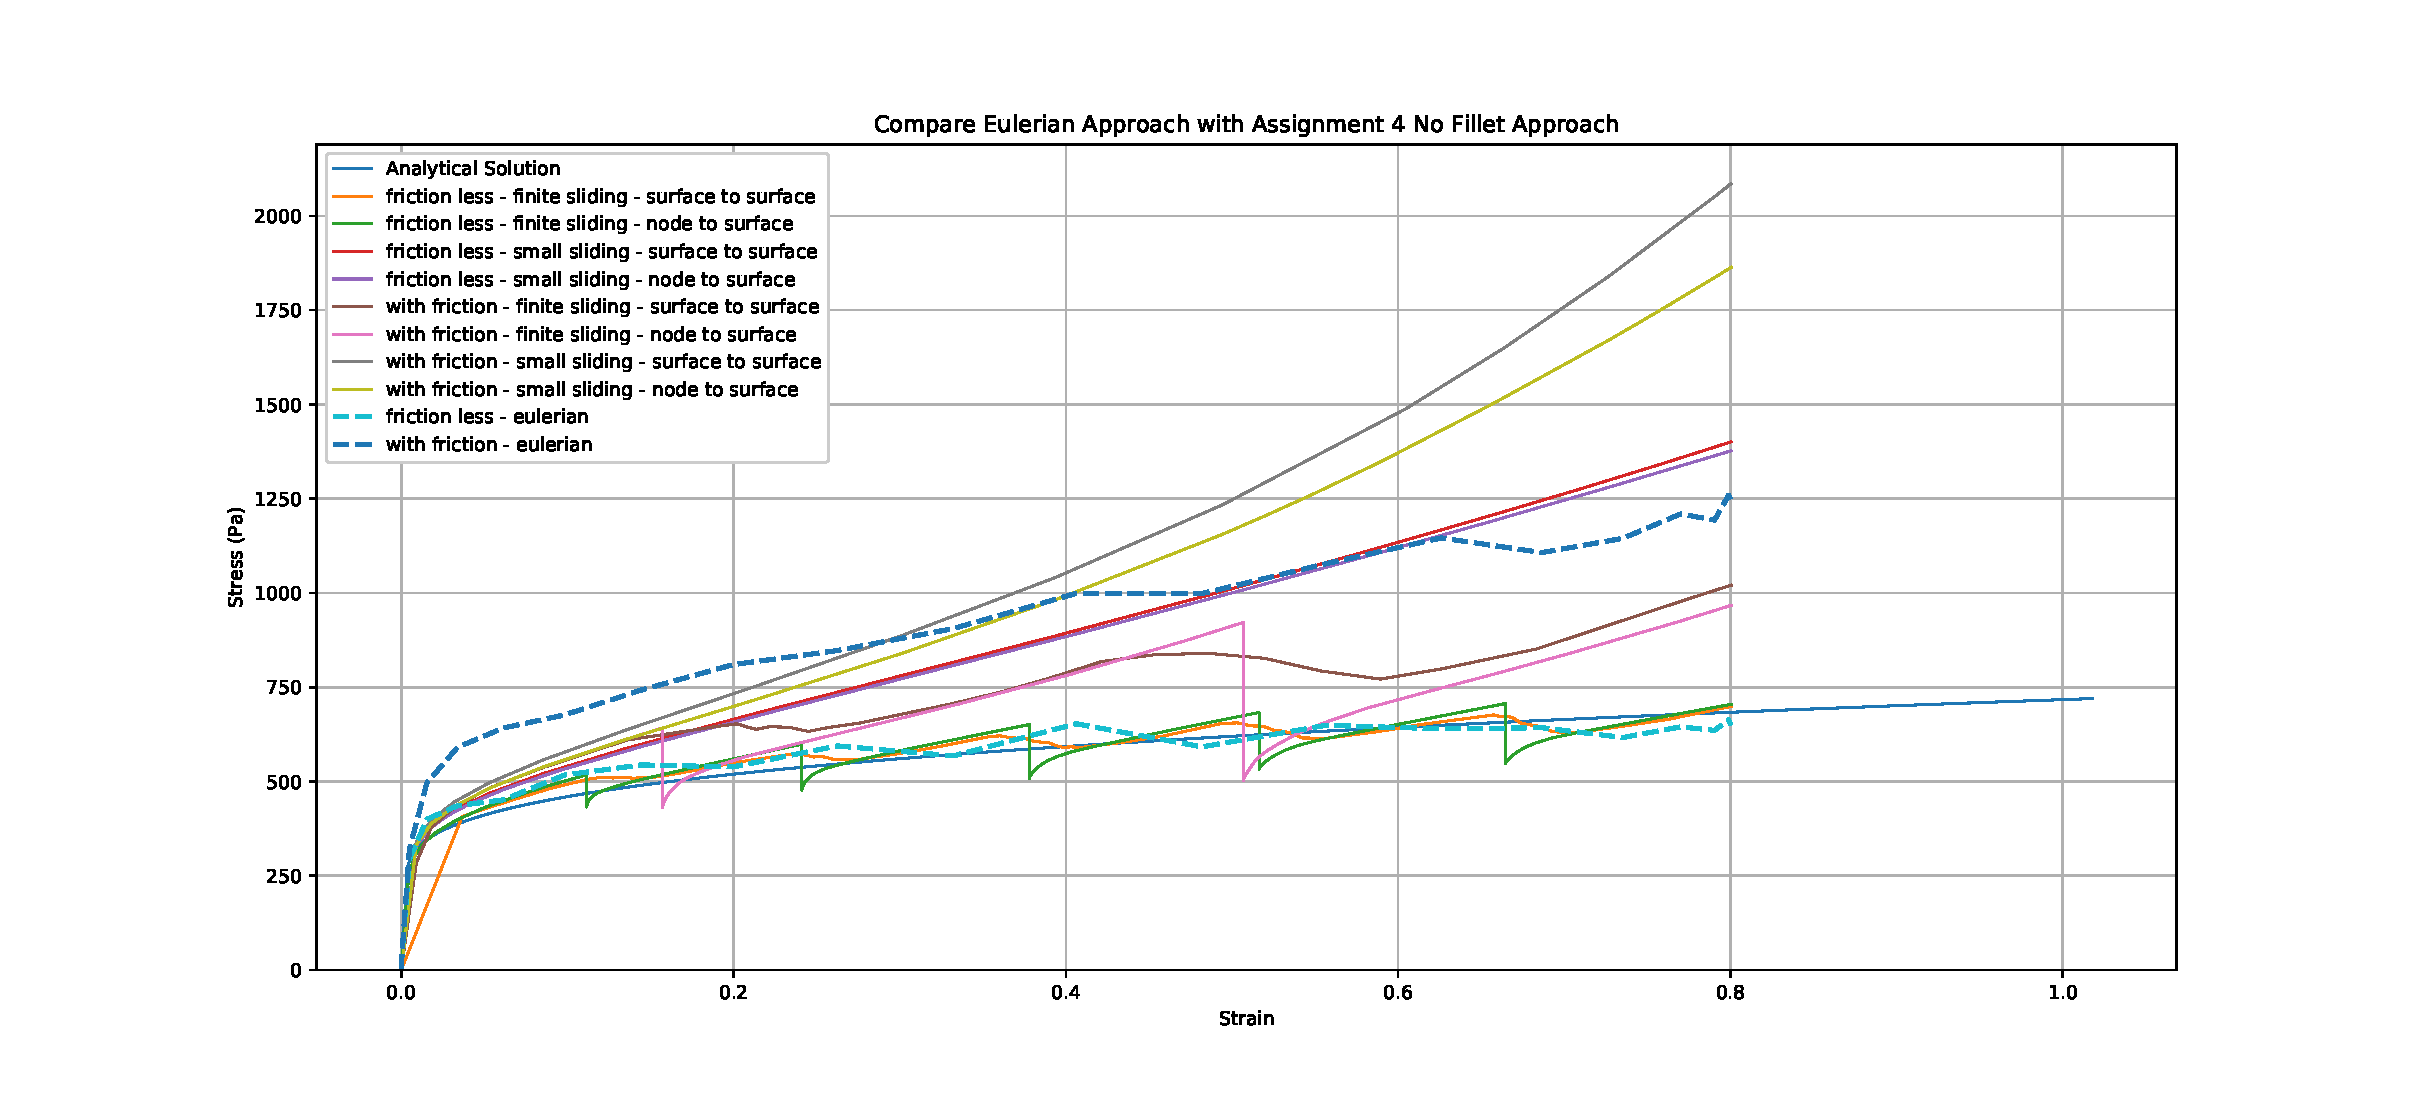
\includegraphics[trim={4cm 1cm 4cm 1.8cm},clip,width=0.9\linewidth]{pics/eulerian_compared}
  \caption{Results of the no fillet model}
  \label{fig:3}
\end{figure}

\newpage

\section{Discussion}

The Eulerian analysis is for simulations with large displacements. The documentation mentions that it can be used effectively with liquid sloshing, gas flow, and penetration problems. Lagrangian elements are easily distorted and lose accuracy, as we saw in the last assignment. For success in the last assignment, tricks have been used, like implementing a fillet and so on.

This is not necessary anymore, in Eulerian analysis, there is no relationship created between the nodes and the surfaces. In fact, the grid stays the same and no deformation of it can be observed. The analysis nodes are fixed in space, the material flows through the elements.

\subsection{No Friction Compairson}

With no friction, the results are similar as in the previous assignment. However, there is a small oscillation visible around the analytical curve. As previously mentioned, the Eulerian analysis is created for simulations with large displacements like water or other liquids. The oscillation is actually the inner forces of the material. The higher the forces, the more likely the forces and displacement are likely to oscillate.

\subsection{Friction Compairson}

One can observe that the curve overshoots much more as with the Lagrangian analysis. Actually, the solution with the Eulerian method is much more accurate. Of course, the mesh density is much higher with the Eulerian method as with the Lagrangian one. As mentioned in the last assignment, the friction property of 0.2 adds additional forces to the simulation. Therefore the additional forces are added to the curve.

\subsection{Explicit Dynamic Analysis}

In general, the explicit dynamics procedure performs many small time increments in a short time. Every time step is dynamically evaluated in order to come forward in the analysis. Also, there is an explicit central-difference operator that tries to satisfy the dynamic equilibrium. Using this approach gives good results in a relatively short time. As we are using a Eulerian model we must also consider the internal forces like in the liquid. Depending on the amplitude of the force this will echo back later, leading in an overshoot or drop in the curve over the time of the curve. The documentation says that this can lead to a problem when the solver is trying to solve for a equilibrium.


\section{Conclusion}

For simulations with large displacement, especially including liquid and gases, the Eulerian analysis is the way to go. In Eulerian analysis, the element can only consist of one material which is good for liquids, as there is only one material necessary, but bad for other model modalities when a part consisting of multiple partitions should also have multiple materials assigned to each partition. Also the documentation of Abaqus many limitations occur in Eulerian analysis, however, a workaround can be found for achieving the same as in Lagrangian in most cases.

\vspace{5mm}
\noindent All information is used from the Abaqus documentation. 

\end{document}